\documentclass[a4paper,11pt]{report}

\usepackage[margin=2.5cm]{geometry}

\usepackage{biblatex}
\addbibresource{citations.bib}

\usepackage{graphicx}
\graphicspath{ {./assets} }

\usepackage{titling}
\usepackage{float}

\usepackage{hyperref}
\hypersetup{
    colorlinks=true,
    linktoc=all,
    citecolor=black,
    % filecolor=black,
    % linkcolor=pink,
    % urlcolor=black
}

\usepackage{minted}
\title{Timber}

\author{
    Reece 119310841
    \and
    Thomas 119429402
    \and
    Shang 119459664
    \and
    Max 119477254
    \and
    Aidan 119456596
}

\title{Timber}
\date{\today}

\begin{document}

\begin{titlepage}
    \begin{center}
        \null
        \vfill
        
        \textbf{Deliverable 1 \& 2}
        \vspace{1cm}

        \large Team 1

        \huge{\thetitle}
        \vspace{0.5cm}

        \normalsize A Collaboration Social Networking Platform

        CS3500 Software Engineering
        \vspace{1cm}


        \today
        \vspace{2cm}
        
        Coordinating Team Member: Thomas Daniel Galligan (119429402)
        \vspace {1cm}

        \theauthor
        \vspace{3cm}


        \textbf{University College Cork}
        
        Ireland
        \vfill

    \end{center}
\end{titlepage}

\cleardoublepage

\begin{abstract}
    Timber is a social networking platform to connect professionals and
    hobbyists together. It’s main purpose is to join people who are looking to
    work on projects in their spare time. It can be ostensible nowadays for a
    student or a person aspiring to join the industry; to find and collaborate
    with and gain team building skills. Our purpose is to mediate these worries
    of finding a team and allow the users to match with each other based on
    their personal similarities and interests. Our goal is to allow people to
    access this in a digestible fashion. Removing high barriers to entry such as
    CVs, lengthy cover letters and experience prerequisites. Users on this
    platform not only can match with these projects but can also use them to
    gain and show their experience on their professional portfolios.
\end{abstract}

\tableofcontents

\chapter{Project Description}

A problem we have all come across has been to find projects to work on to build
our portfolio or to get experience. The project we have chosen is a project and
team matching platform called Timber. Named Timber due to its uses in building
projects. Timber is a platform for aspiring collaborators and project owners to
find the perfect team and project to work on. Collaborators can sign up and
enter their skills. Project Owners can sign up and create their project, and
enter what type of skills prospective collaborators need to be matched with this
project and receive a list of suitable collaborators they can accept or reject.

\chapter{Market Research}
The aim of this project stems from our own experience as students (focusing on
software development) and new developers. It can often be quite difficult to
find group projects to work on to gain developer experience and experience as
part of a team to product a project. A great barrier of entry to these prospects
is often prior experience in these fields, which creates an unfortunate
Catch-22\footnote{Catch-22 - a  situation from which an individual cannot escape
because of contradictory rules or limitations}. This project aims to bridge the
gap, allowing new developers to gain experienece in team-based projects with
minimal background, in the hopes to allow the user to gain experience, which
will allow them entry to job interviews with CVs detailing their experiences.
According to a \href{https://insights.stackoverflow.com/survey/2021#work}{Stack
Overflow Survey in 2021}, 22\% of those who took the survey are either students or
unemployed, which make a good target demographic for this project.

As it stands, there is likely no competitors for this market with this aim, as
when searching for web results for "Getting involved in programming projects"
the main relevant result is Quora articles
[\href{https://www.quora.com/How-can-I-get-developers-to-collaborate-on-my-project-on-GitHub}{How
can I get developers to collaborate on my project on GitHub},
\href{https://www.quora.com/Where-can-I-find-like-minded-programmers-to-collaborate-on-a-project}{Where
can I find like-minded programmers to collaborate on a project}]. The only
somewhat relevant competitor worthy of note is Github Expore. Github Explore is
a service in Github that allows users browse popular and (perhaps) relevant
Open-Source projects to collaborate to. However, this recommends already
in-development projects that may overwhelm new developers, with a large codebase
and large amount of collaborators constantly changing the project's structure
and code. Timber, on the other hand, aims to help new developers start on a
(generally) new project with low barrier of entry, with a (generally) small
developement team, so that collaborators can discuss how to contribute and how
development is going at any given time.

In conclusion, from performing online research of the market, there is
enthusiasm to work on projects to gain experience, but the  barrier of entry can
be considerably high with competitors for this market, but Timber aims to extend
a helping hand to help new developers find their way.

\chapter{Use Cases}
\begin{enumerate}
    \item Users can Login and Register
    \item Two user types: Project Owner and Collaborator (an account can be both)
    \item Project Owner creates and manages a project in the hopes to form a
    team of Collaborators

    \item Project Owner defines required and “wanted” skills/tags on a project
    to attract specific Collaborators

    \item A Collaborator is shown projects relative to their skills/tags in a
    “stack” of projects, which they can “apply to” or dismiss with minimal input
    \item Project Owner is shown Collaborator applicants in a “stack” of users,
    which can be accepted or dismissed with minimal input

    \item Collaborators can “browse” popular/trending projects

    \item Project Owners \& Collaborators can create and edit their profile. A
    Collaborators’s profile can be seen by a Project Owner who has received an
    application from them. A Project Owner’s profile can be seen by
    Collaborator’s who is trying to match with their project

    \item Collaborators can apply to a project, if they match the required
    skills/tags to apply.

    \item Project Owner can accept a collaborator after perusing the Collaborator’s profile
\end{enumerate}

\section{Use Case Diagram}
A use case is a narrative about a user's interaction with a system or
application that captures a set of related behaviors. This narrative is the
context that shapes the design of the system or application. In this UML
visualization , Use cases are split into two types: Project Owner and
Collaborator, both can login, create and manage a project with the hope of
finding the right Collaborator to join the team. The Collaborator is shown
projects relative to their skills/tags or can browse popular/trending projects
in hopes of finding one they are interested in, and may apply to. If the Project
Owner receives an application, the Collaborator’s profile is visible. If the
Project Owner is interested, they can accept the Collaborator.

\begin{figure}[H]
    \centering
    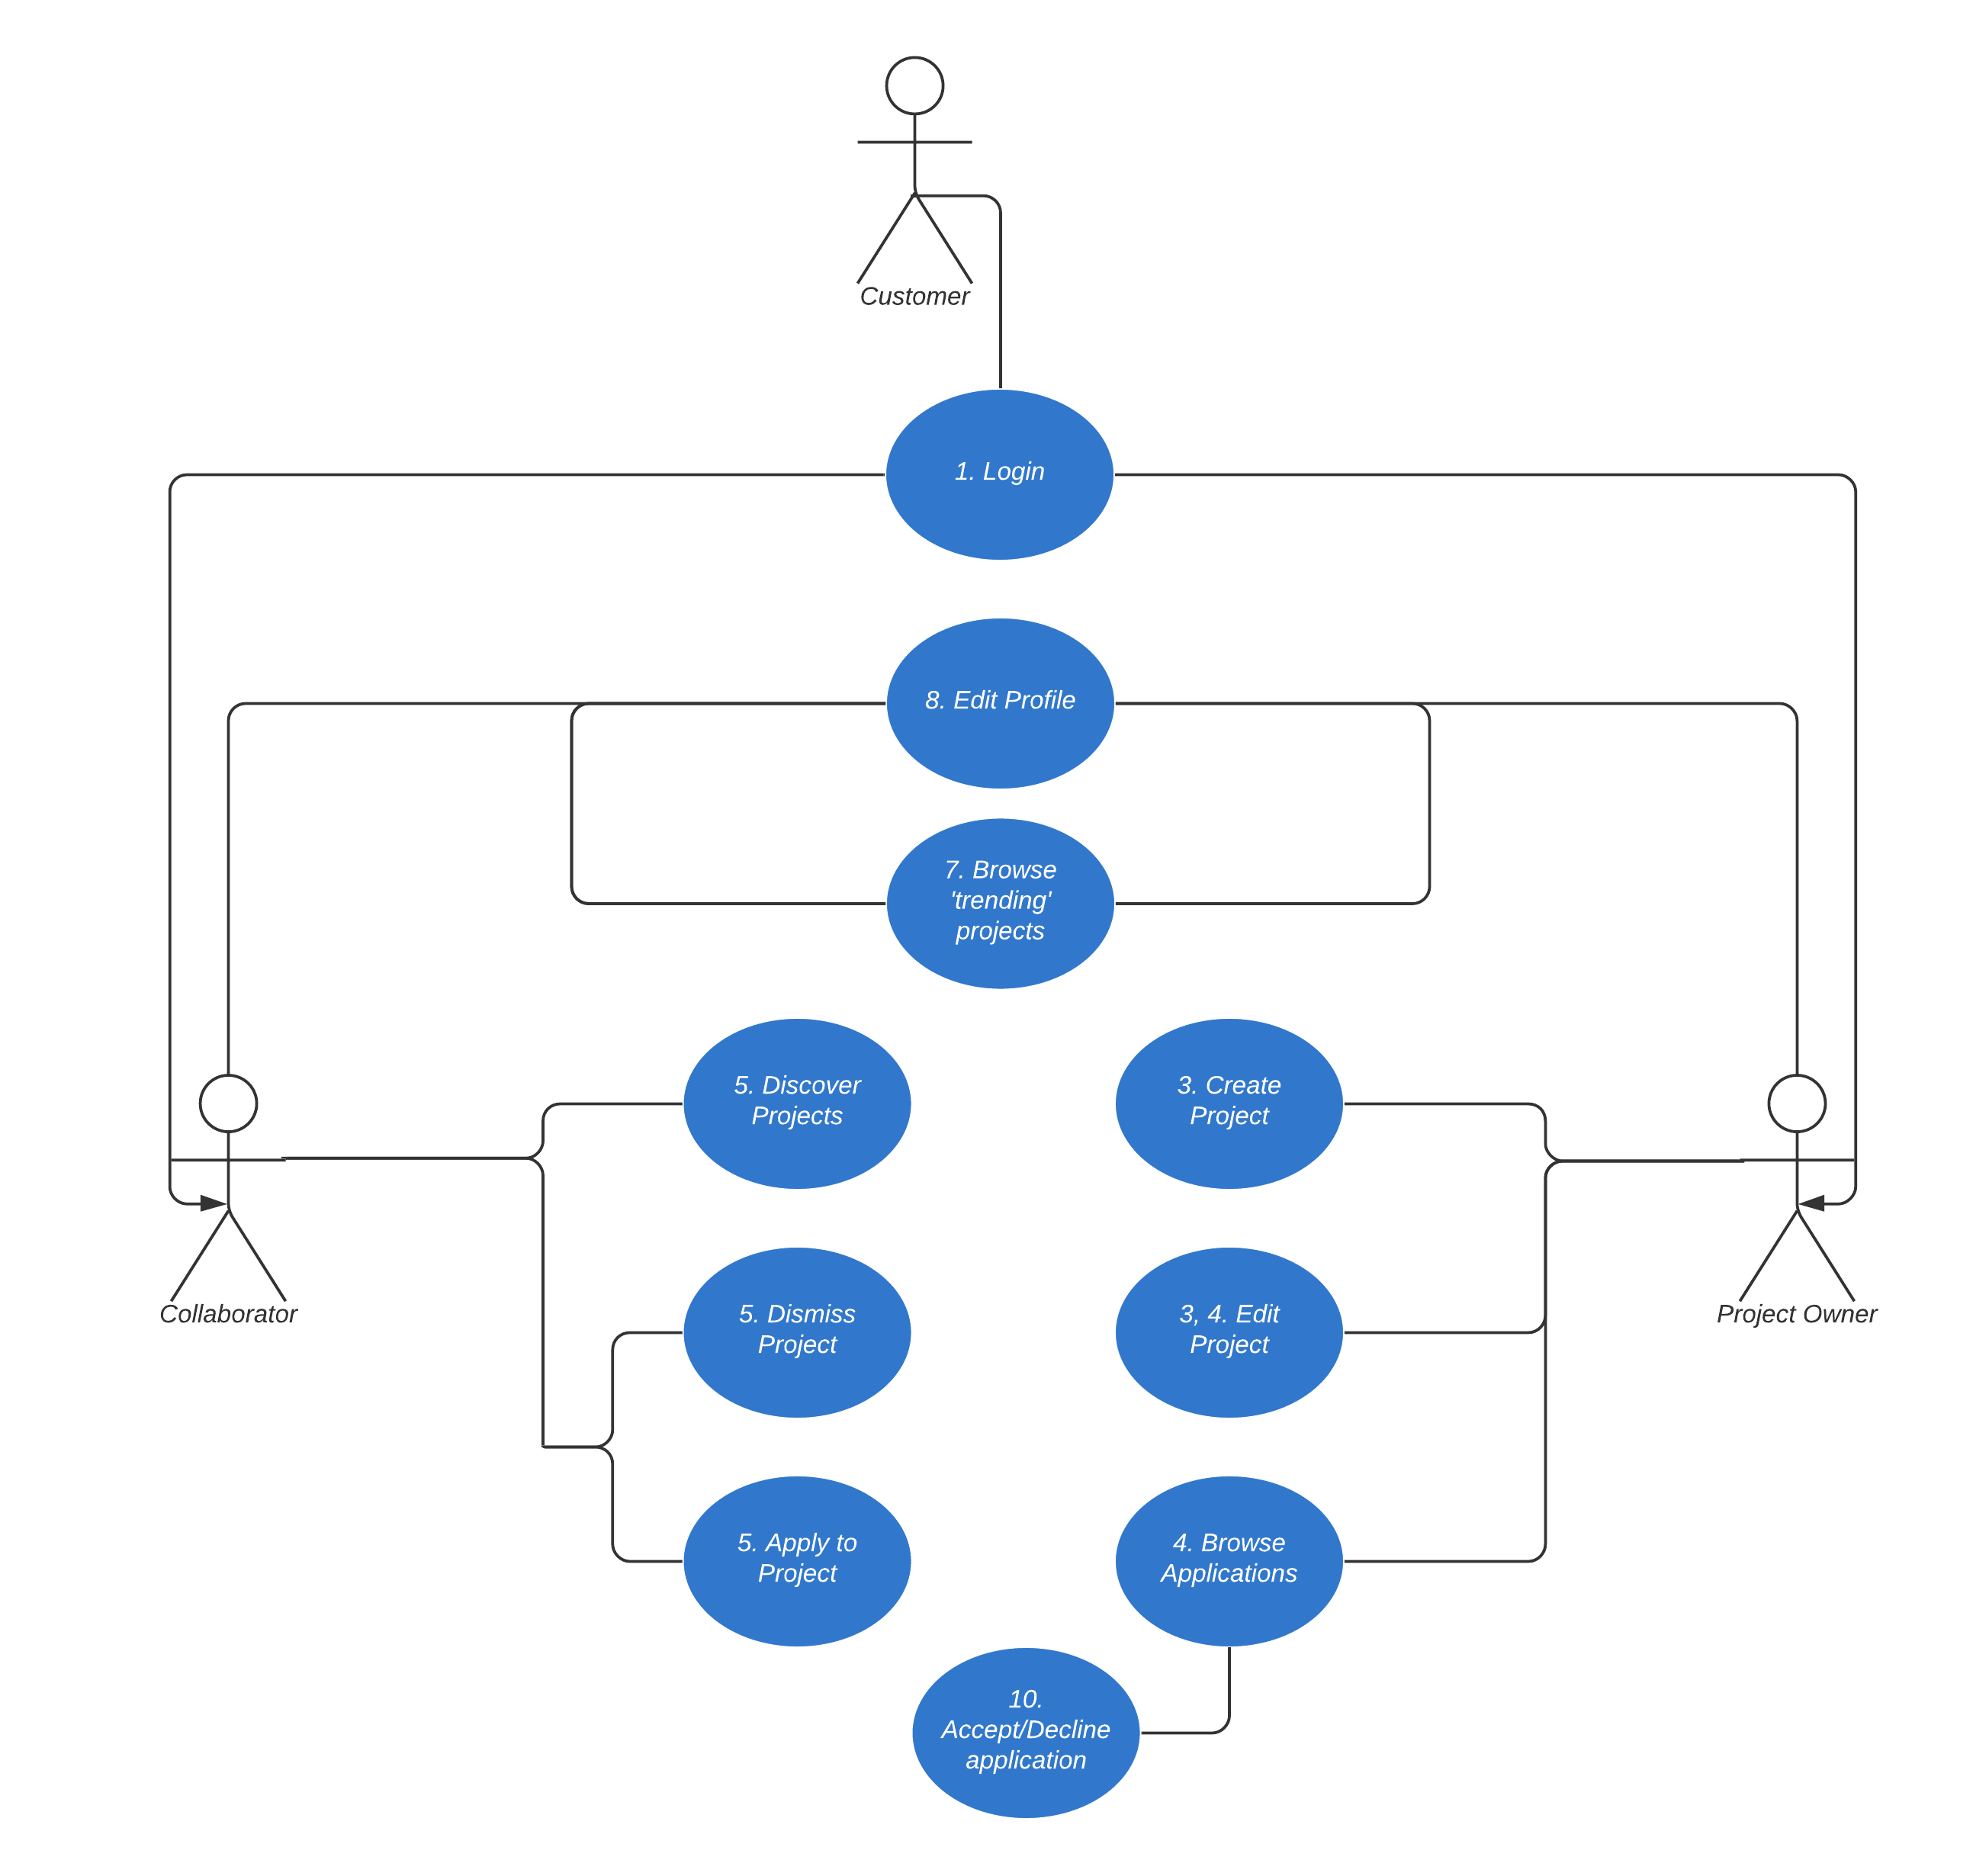
\includegraphics[width=\textwidth,height=\textheight,keepaspectratio]{usecasediagram.png}
    \caption{Use Case Diagram}
    \label{fig:usecase}
    \
\end{figure}

\newpage
\section{Collaborator State-Transition diagram}
This state-transition diagram demonstrates how a user acting as a Collaborator
may interact and use this product. It details how a Collaborator may apply to
Projects and check the status of their applications before accepting the
invitation to collaborate.

\begin{figure}[H]
    \centering
    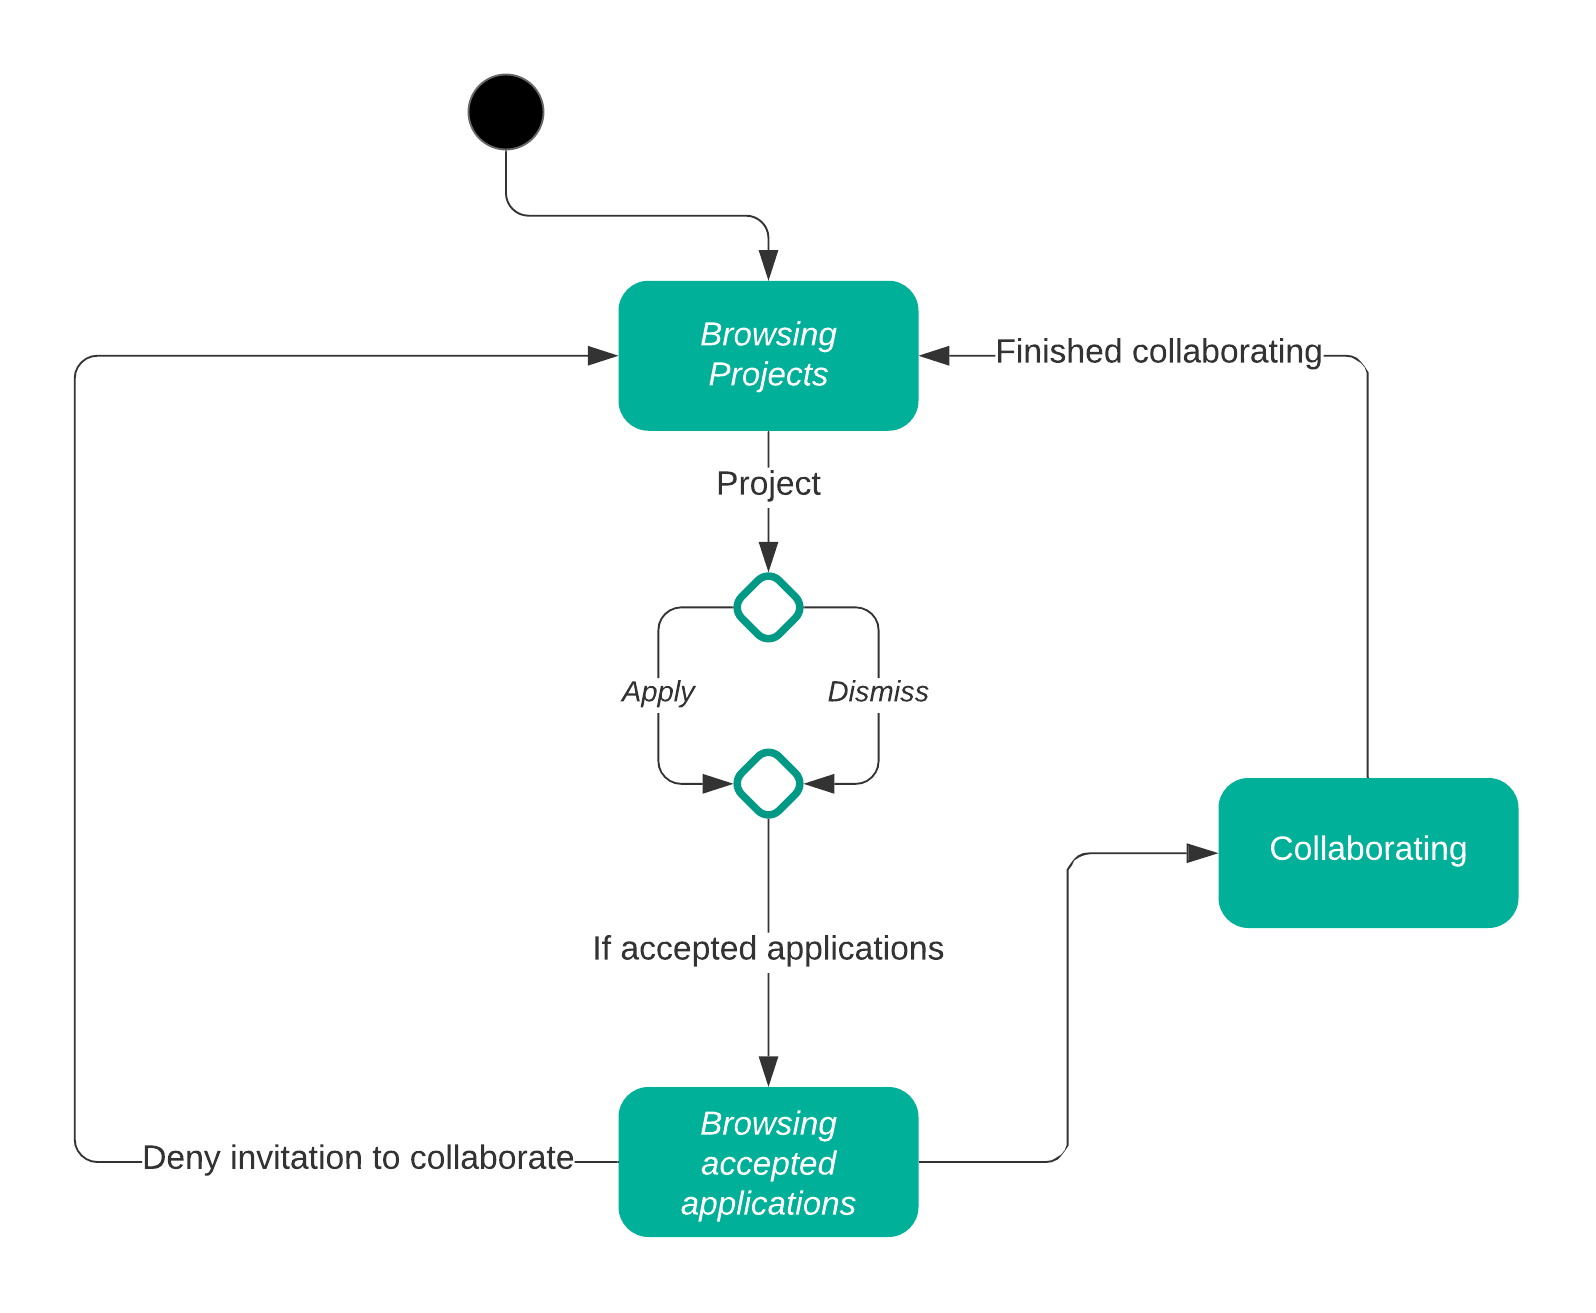
\includegraphics[width=0.9\textwidth,keepaspectratio]{std-collaborator.png}
    \caption{Collaborator State-Transition Diagram}
    \label{fig:collaborator-std}
\end{figure}

\section{Project Owner State-Transition Diagram}
This state-transition diagram demonstrates how a user acting as a Project Owner
may interact and use this product. It details how a user may go about creating
and managing a Project, and how they may accept and deny applications before
commencing work on a project when enough Collaborators are accepted.

\begin{figure}[h]
    \centering
    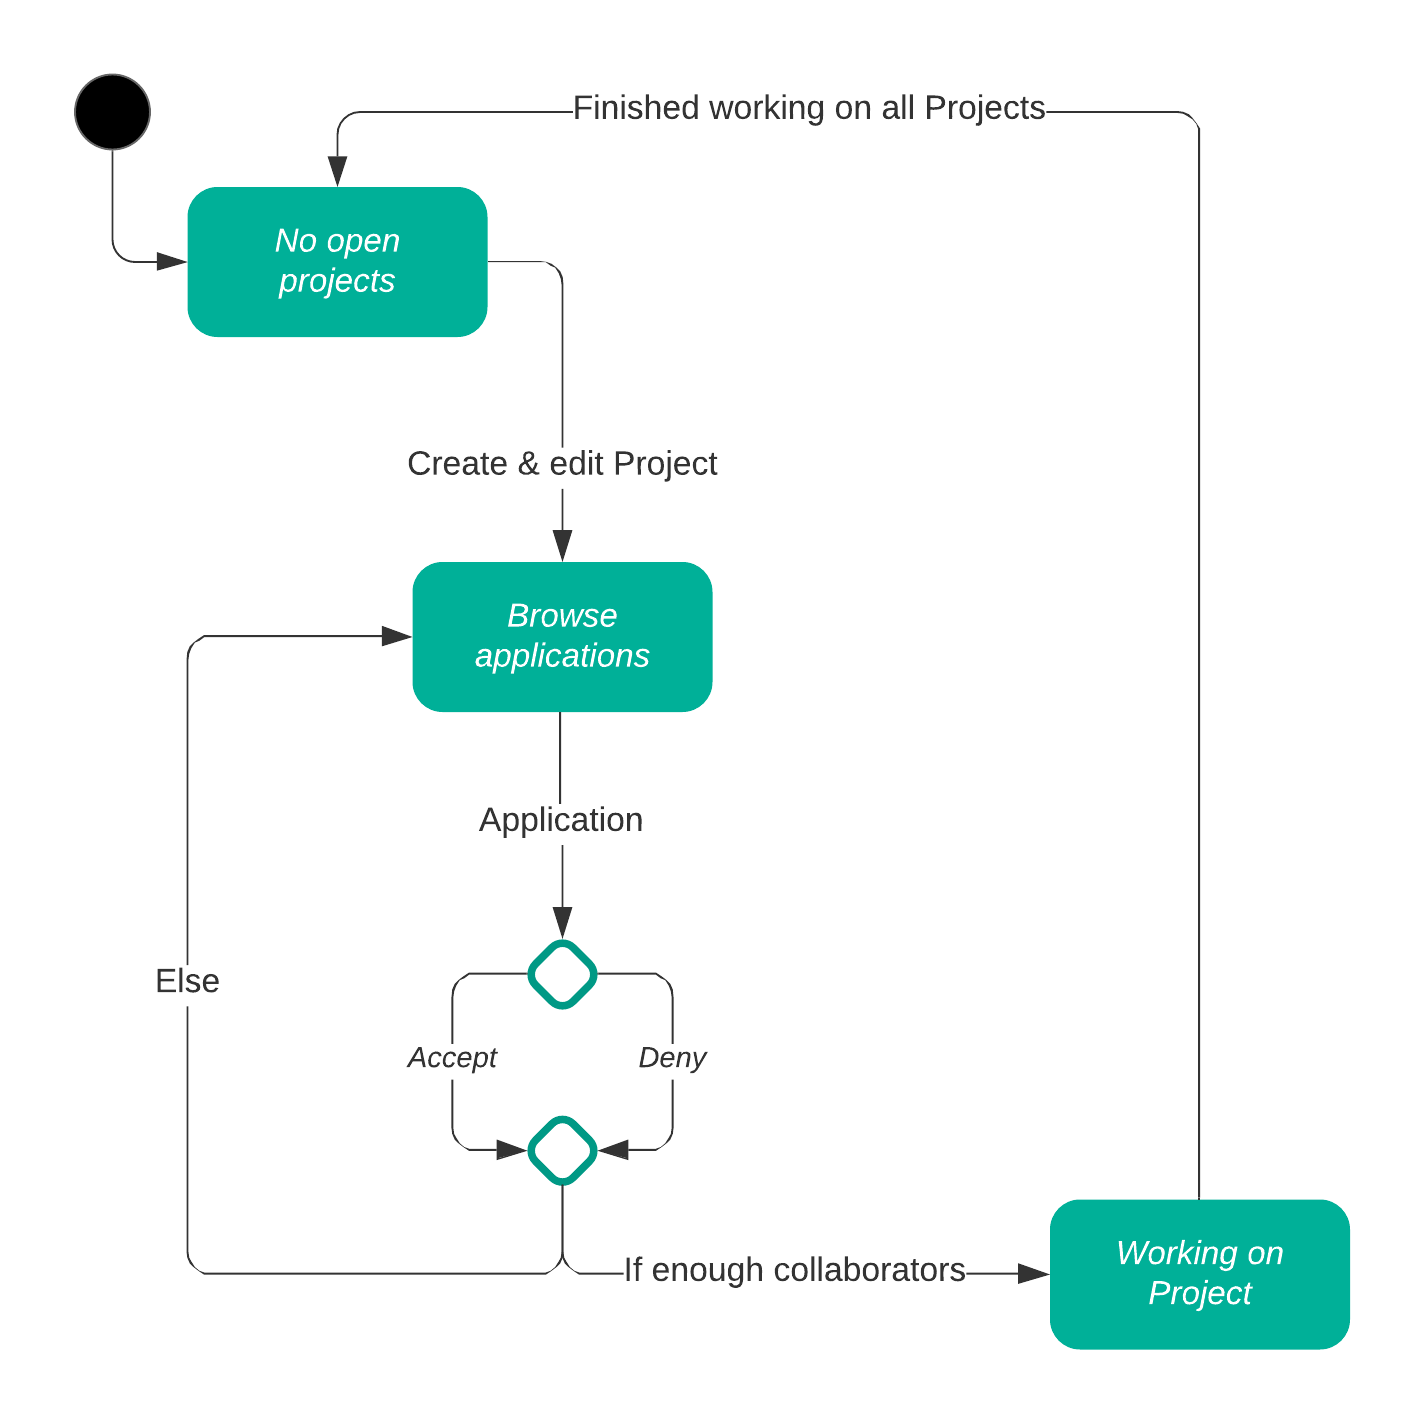
\includegraphics[width=0.9\textwidth,keepaspectratio]{std-projectowner.png}
    \caption{Project Owner State-Transition Diagram}
    \label{fig:projectowner-std}
\end{figure}

\chapter{Requirements}
\section{Back-End}
\begin{enumerate}
    \item Choose and set up a database which can handle a high-volume of queries
    and is scalable before starting development on the back-end

    \item The back-end must be able to be hosted on the cloud, and be
    cloud-agnostic to allow for scalability and avoid being “locked-in” to
    specific cloud companies. This also means the code must be capable of
    running on different operating systems, and with few compute resources - ie.
    small memory pool. This should be considered throughout development, but
    especially before choosing language/frameworks to account for this.

    \item The back-end must be capable of handling large volumes of traffic, and
    make fast responses to clients. This must be considered whenever adding a
    feature, changing a feature of the back-end.

    \item Authentication/Authorization must be secure, to protect user data.
    While also being scalable and fast. This is vitally-important, and must be
    implemented immediately upon creating the first back-end API route, or even
    earlier.
\end{enumerate}

\section{Front-End}
\begin{enumerate}
    \item Front-end must be usable on most modern browsers, ( \textgreater IE 11 ). This
    must be considered throughout development. However, special consideration
    should be taken into account when choosing frameworks/libraries (2), so as
    to ensure maximum compatibility.

    \item Front-end should be based on a mobile-first design. A common use-case
    of this product is in situations without access to a personal computer.
    These users should be considered as first class users and the interface
    designed around them accordingly. This should be at the forefront of
    developers minds throughout the front-end design process.

    \item Front-end must make use of frameworks/libraries to speed up
    development time. This should be decided on before writing any front-end
    code.

    \item Front-end should make use of wireframes to draft-out UI components
    before writing them in code. This is to allow developers to visualize the UI
    before taking time to manually create the components in code. This should be
    done throughout front-end development.

    \item An SDK/library must be created as soon as the backend API is in some
    working state. This will create a simple and standardised way for the
    front-end to interact with the back-end, to create a centralised place for
    the process of code testing and code verification. All front-end to back-end
    interactions should use this library.

    \item Front-end should be an accessible and easy to use design. It should
    not use design concepts that require too much thought. This ease of use
    improves user interaction and retention with the service. It also ensures
    that those with an impairment have as good as possible experience with the
    product. This should be kept in mind as much as possible during
    implementation and design of the front-end
\end{enumerate}

\chapter{Data Flow Diagrams}
The following Data-Flow diagrams are to demonstrate how data is passed around
and transferred between processes and entities in our tech stack. These are
represented in "levels", depciting increasingly complex and lower-level views of
how the tech stack works.

\section{Data Flow Diagram Level 0}
\begin{figure}[h]
    \centering
    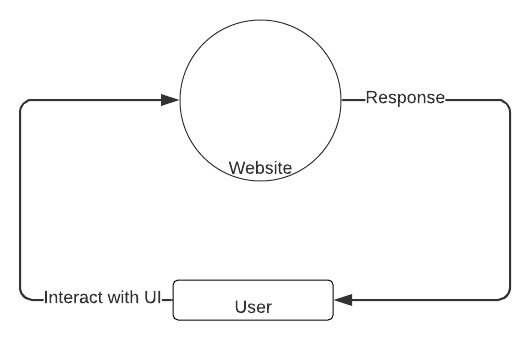
\includegraphics[width=0.5\textwidth,keepaspectratio]{d2-dfd-0.png}
    \caption{Data flow diagram Level 0}
    \label{fig:dfd-0}
\end{figure}

A very simple overview of how data flows through the app can be seen in
\ref{fig:dfd-0}, where a user interacts with a website, using the UI to abstract
away the inner-workings of the system. The user is presented with feedback as a
response through the user interface of the website.

\newpage
\section{Data Flow Diagram Level 1}
\begin{figure}[h]
    \centering
    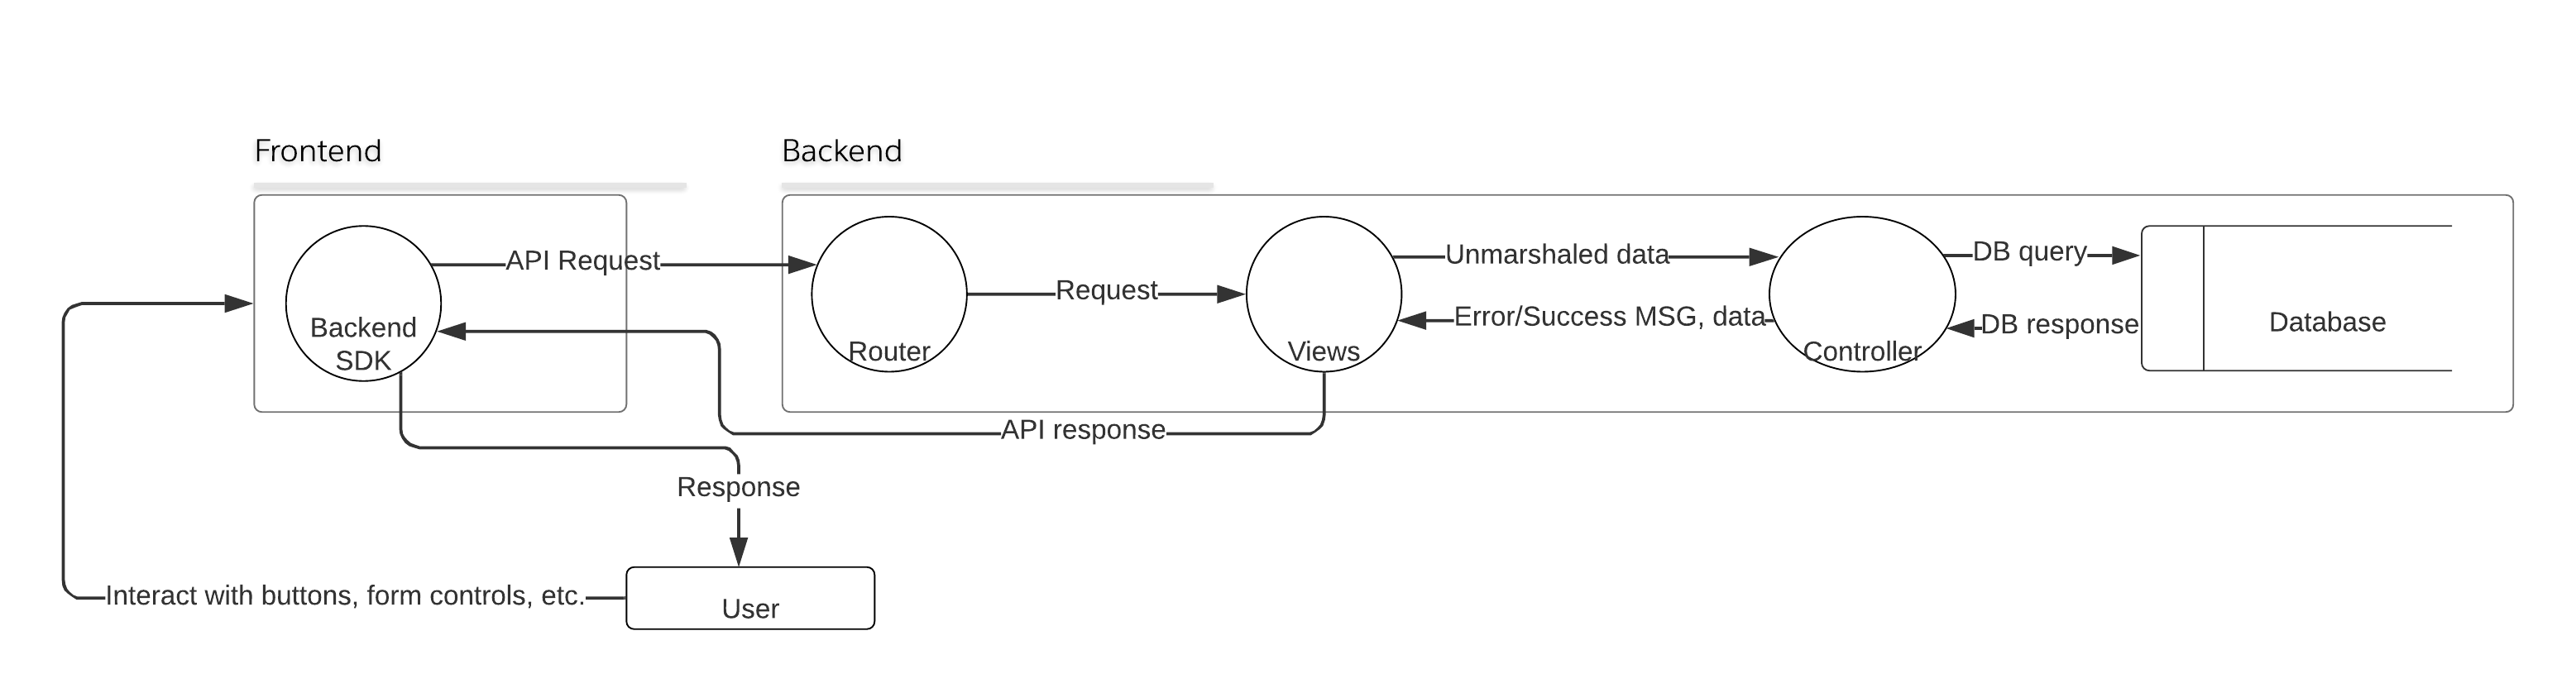
\includegraphics[width=\textwidth]{d2-dfd-1.png}
    \caption{Data flow diagram Level 1}
    \label{fig:dfd-1}
\end{figure}

A more complex and truthful overview of how data moves through the system is
demonstrated in \ref{fig:dfd-1}, showing a bridge between frontend and backend,
where a user's interaction with the backend is abstracted by the frontend. The
"Router" process routes a request to relevant handler, located in "Views"
process, which unmarshals data sent in request and calls on "Controller" to
modify and request data from database. Most data manipulation and storage
occcurs in the backend.

\section{Data Flow Diagram Level 2}
\begin{figure}[h]
    \centering
    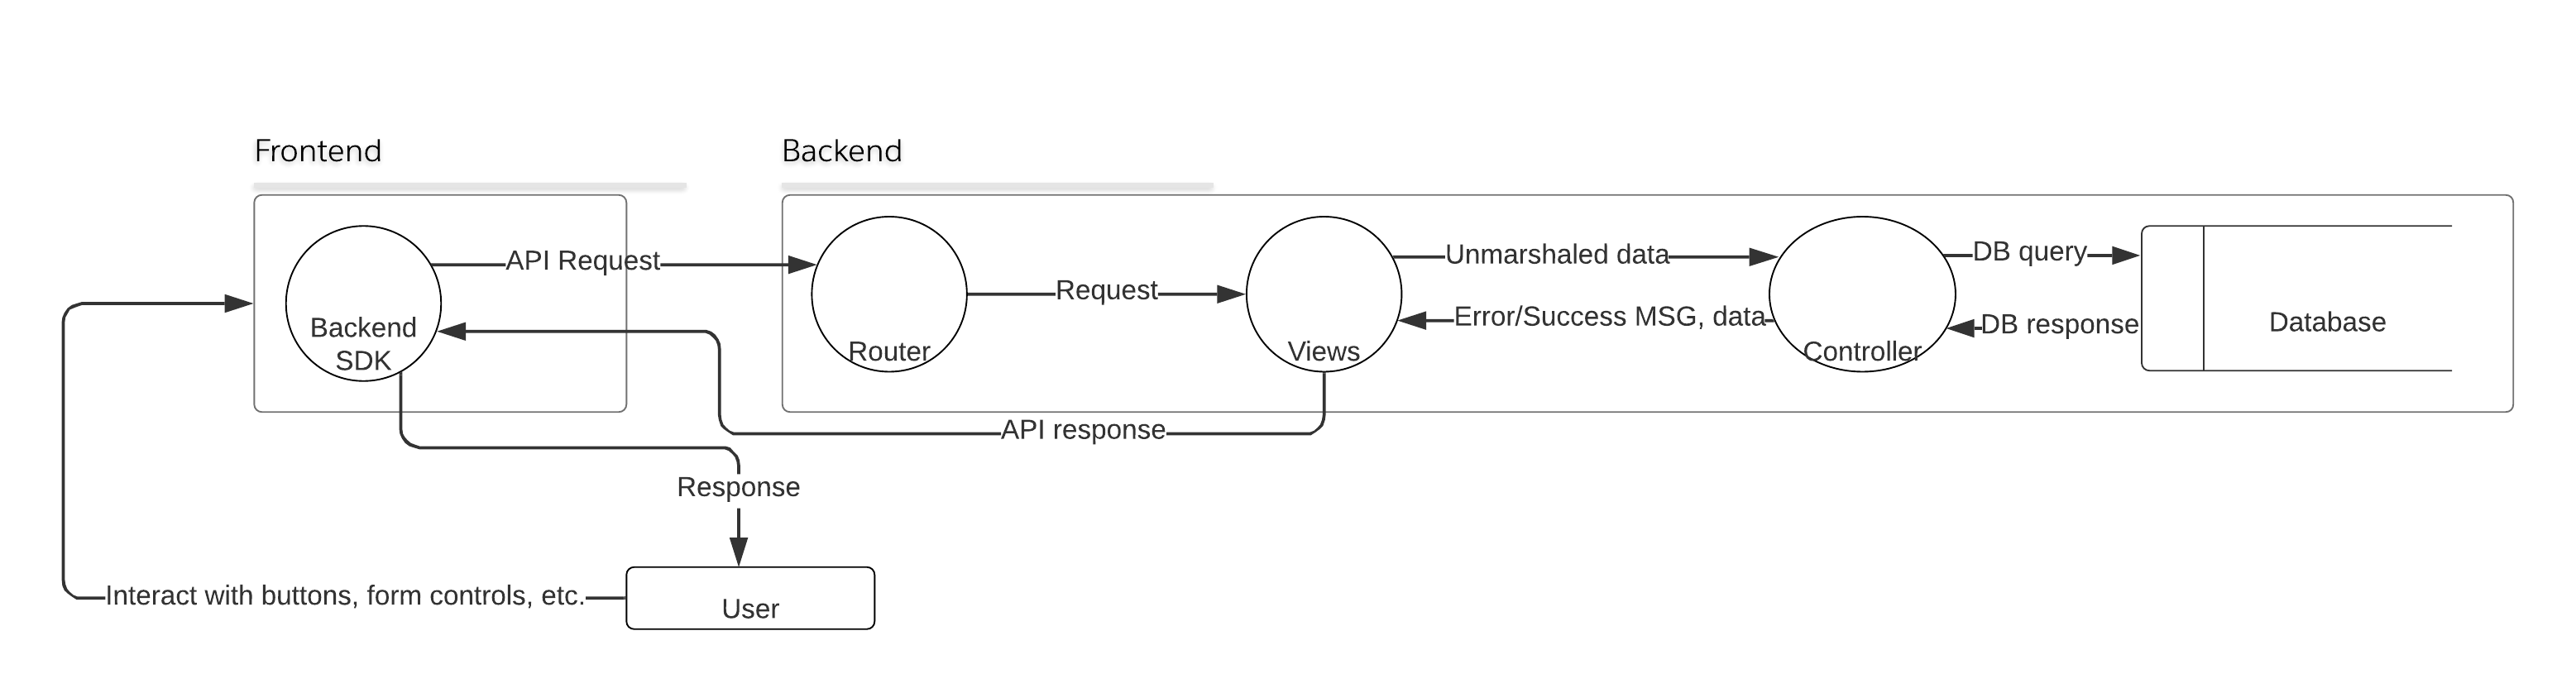
\includegraphics[width=\textwidth]{d2-dfd-2.png}
    \caption{Data flow diagram Level 2}
    \label{fig:dfd-2}
\end{figure}

Once again, an even more in-depth diagram can be seen at \ref{fig:dfd-2},
detailing the use of middleware for logging processed requests, and checking
authorization headers of incoming requests, and tagging a request with the
user's ID before continuing on to the "Views" process. Also, we can see how our
"Stores" process interacts with a database, proxying and creating database
queries called from our "Controllers".

\newpage
\section{Sequence Diagrams}
Sequence diagrams help demonstrate how a user interacts with a service, and how
this service interacts with other services in the system.

\begin{figure}[H]
    \centering
    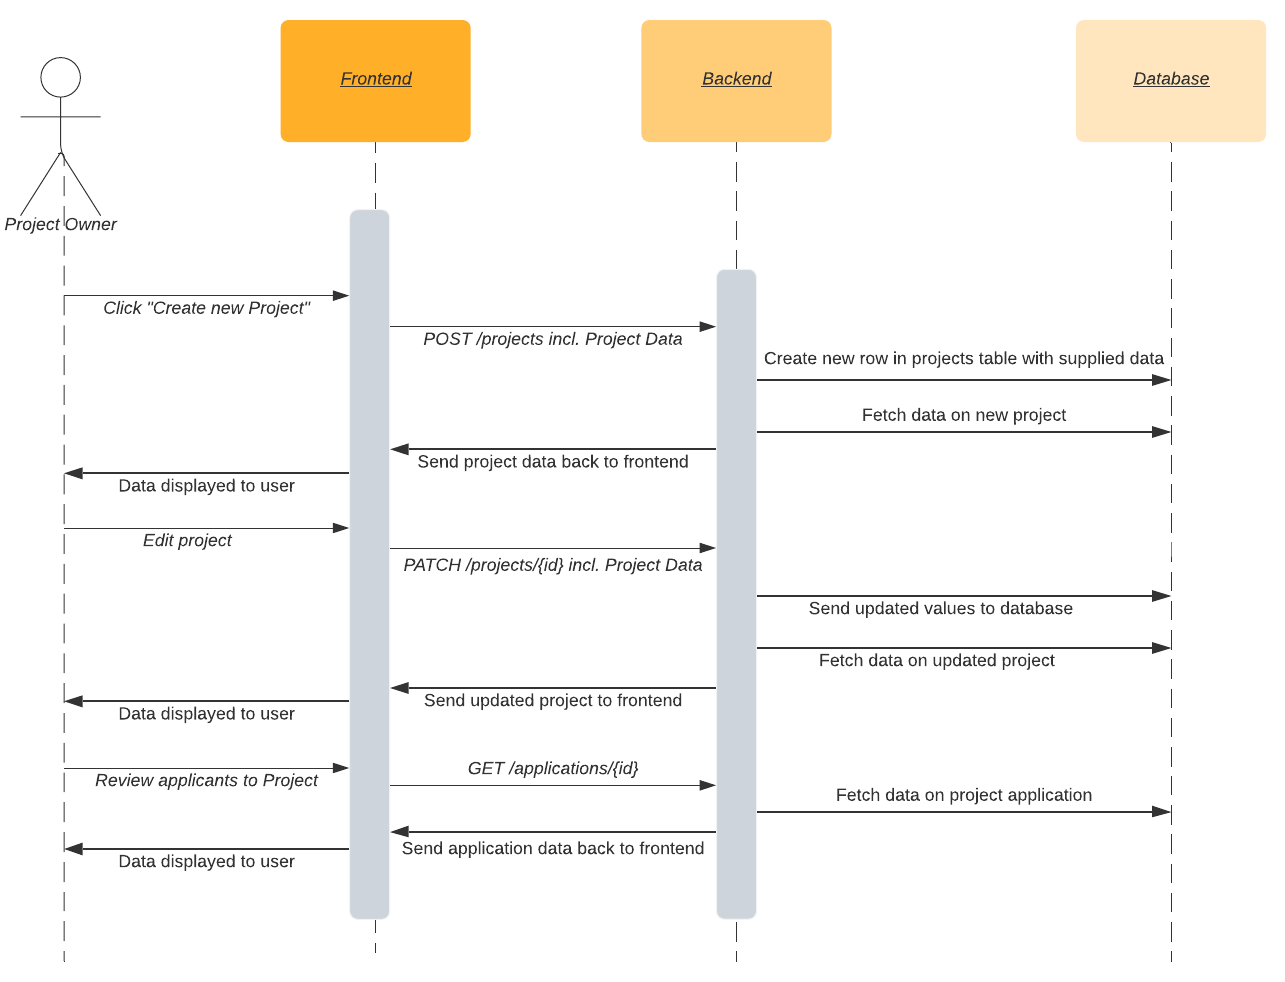
\includegraphics[width=\textwidth]{sd-projectowner.png}
    \caption{Project Owner Sequence Diagram}
    \label{fig:projectowner-sd}
\end{figure}

\begin{figure}[H]
    \centering
    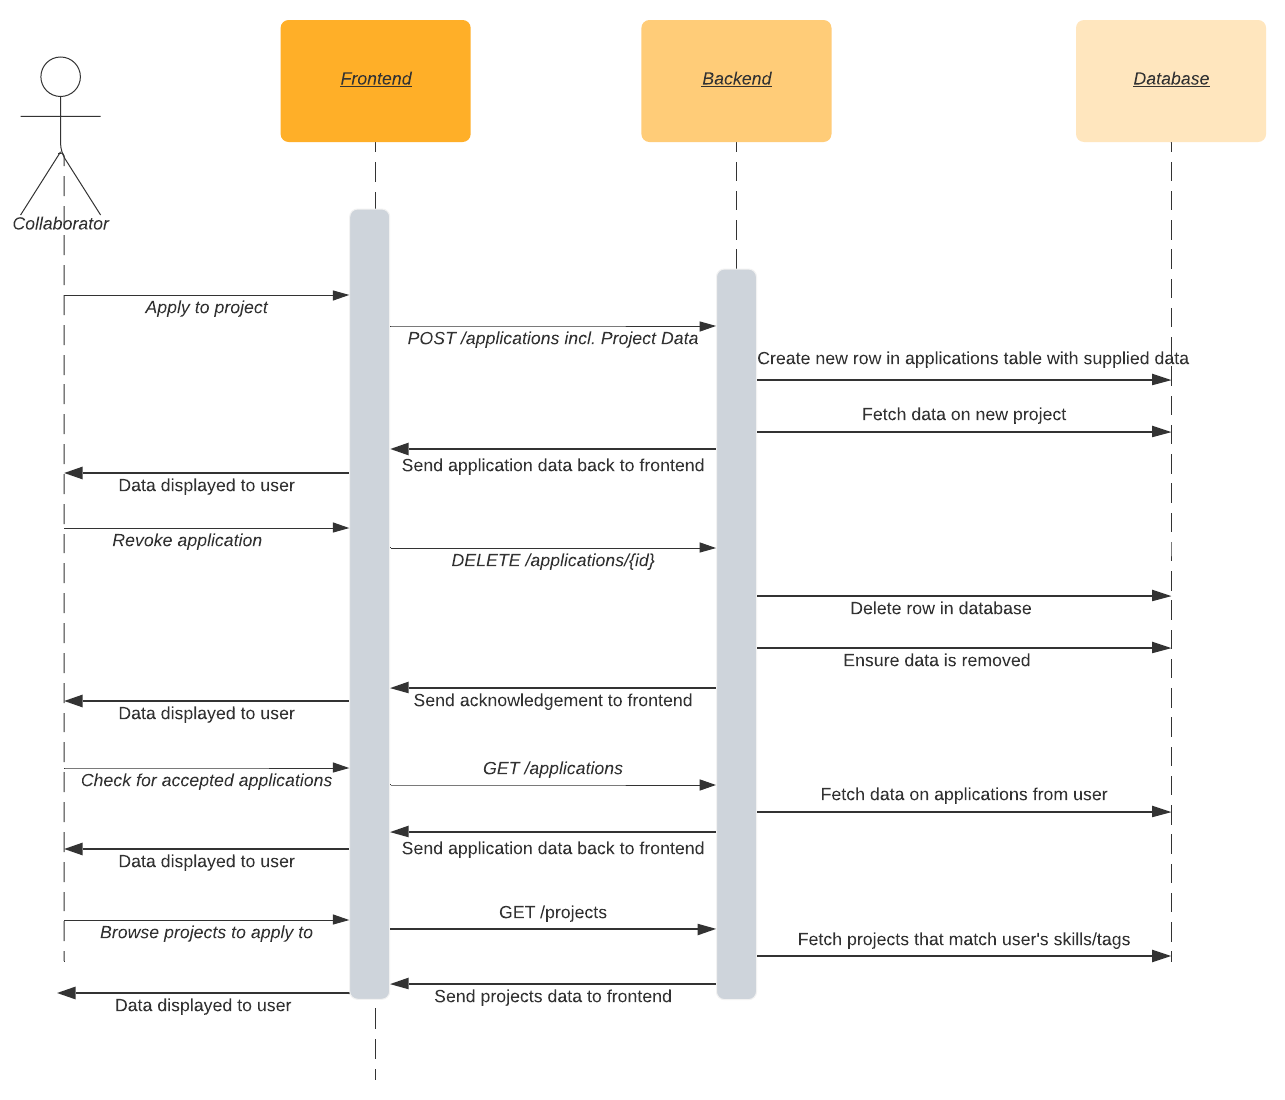
\includegraphics[width=\textwidth,keepaspectratio]{sd-collaborator.png}
    \caption{Collaborator Sequence Diagram}
    \label{fig:collaborator-sd}
\end{figure}


As can be seen in both \ref{fig:projectowner-sd} and \ref{fig:collaborator-sd},
a user directly interacts with the frontend or UI, which in turn interfaces with
the backend, or API. This api then manipulates and processes data sent by the
user in the frontend, and stores this data in the database, before fetching
updated data and returning it to the frontend, which is displayed visually to
the user.

\chapter{Implementation Detail}
As the complexity of the backend is considerable, it is worth describing the
requirements and purpose of each process detailed in the Backend Overview
\ref{fig:backend-overview}

\begin{figure}[b]
    \centering
    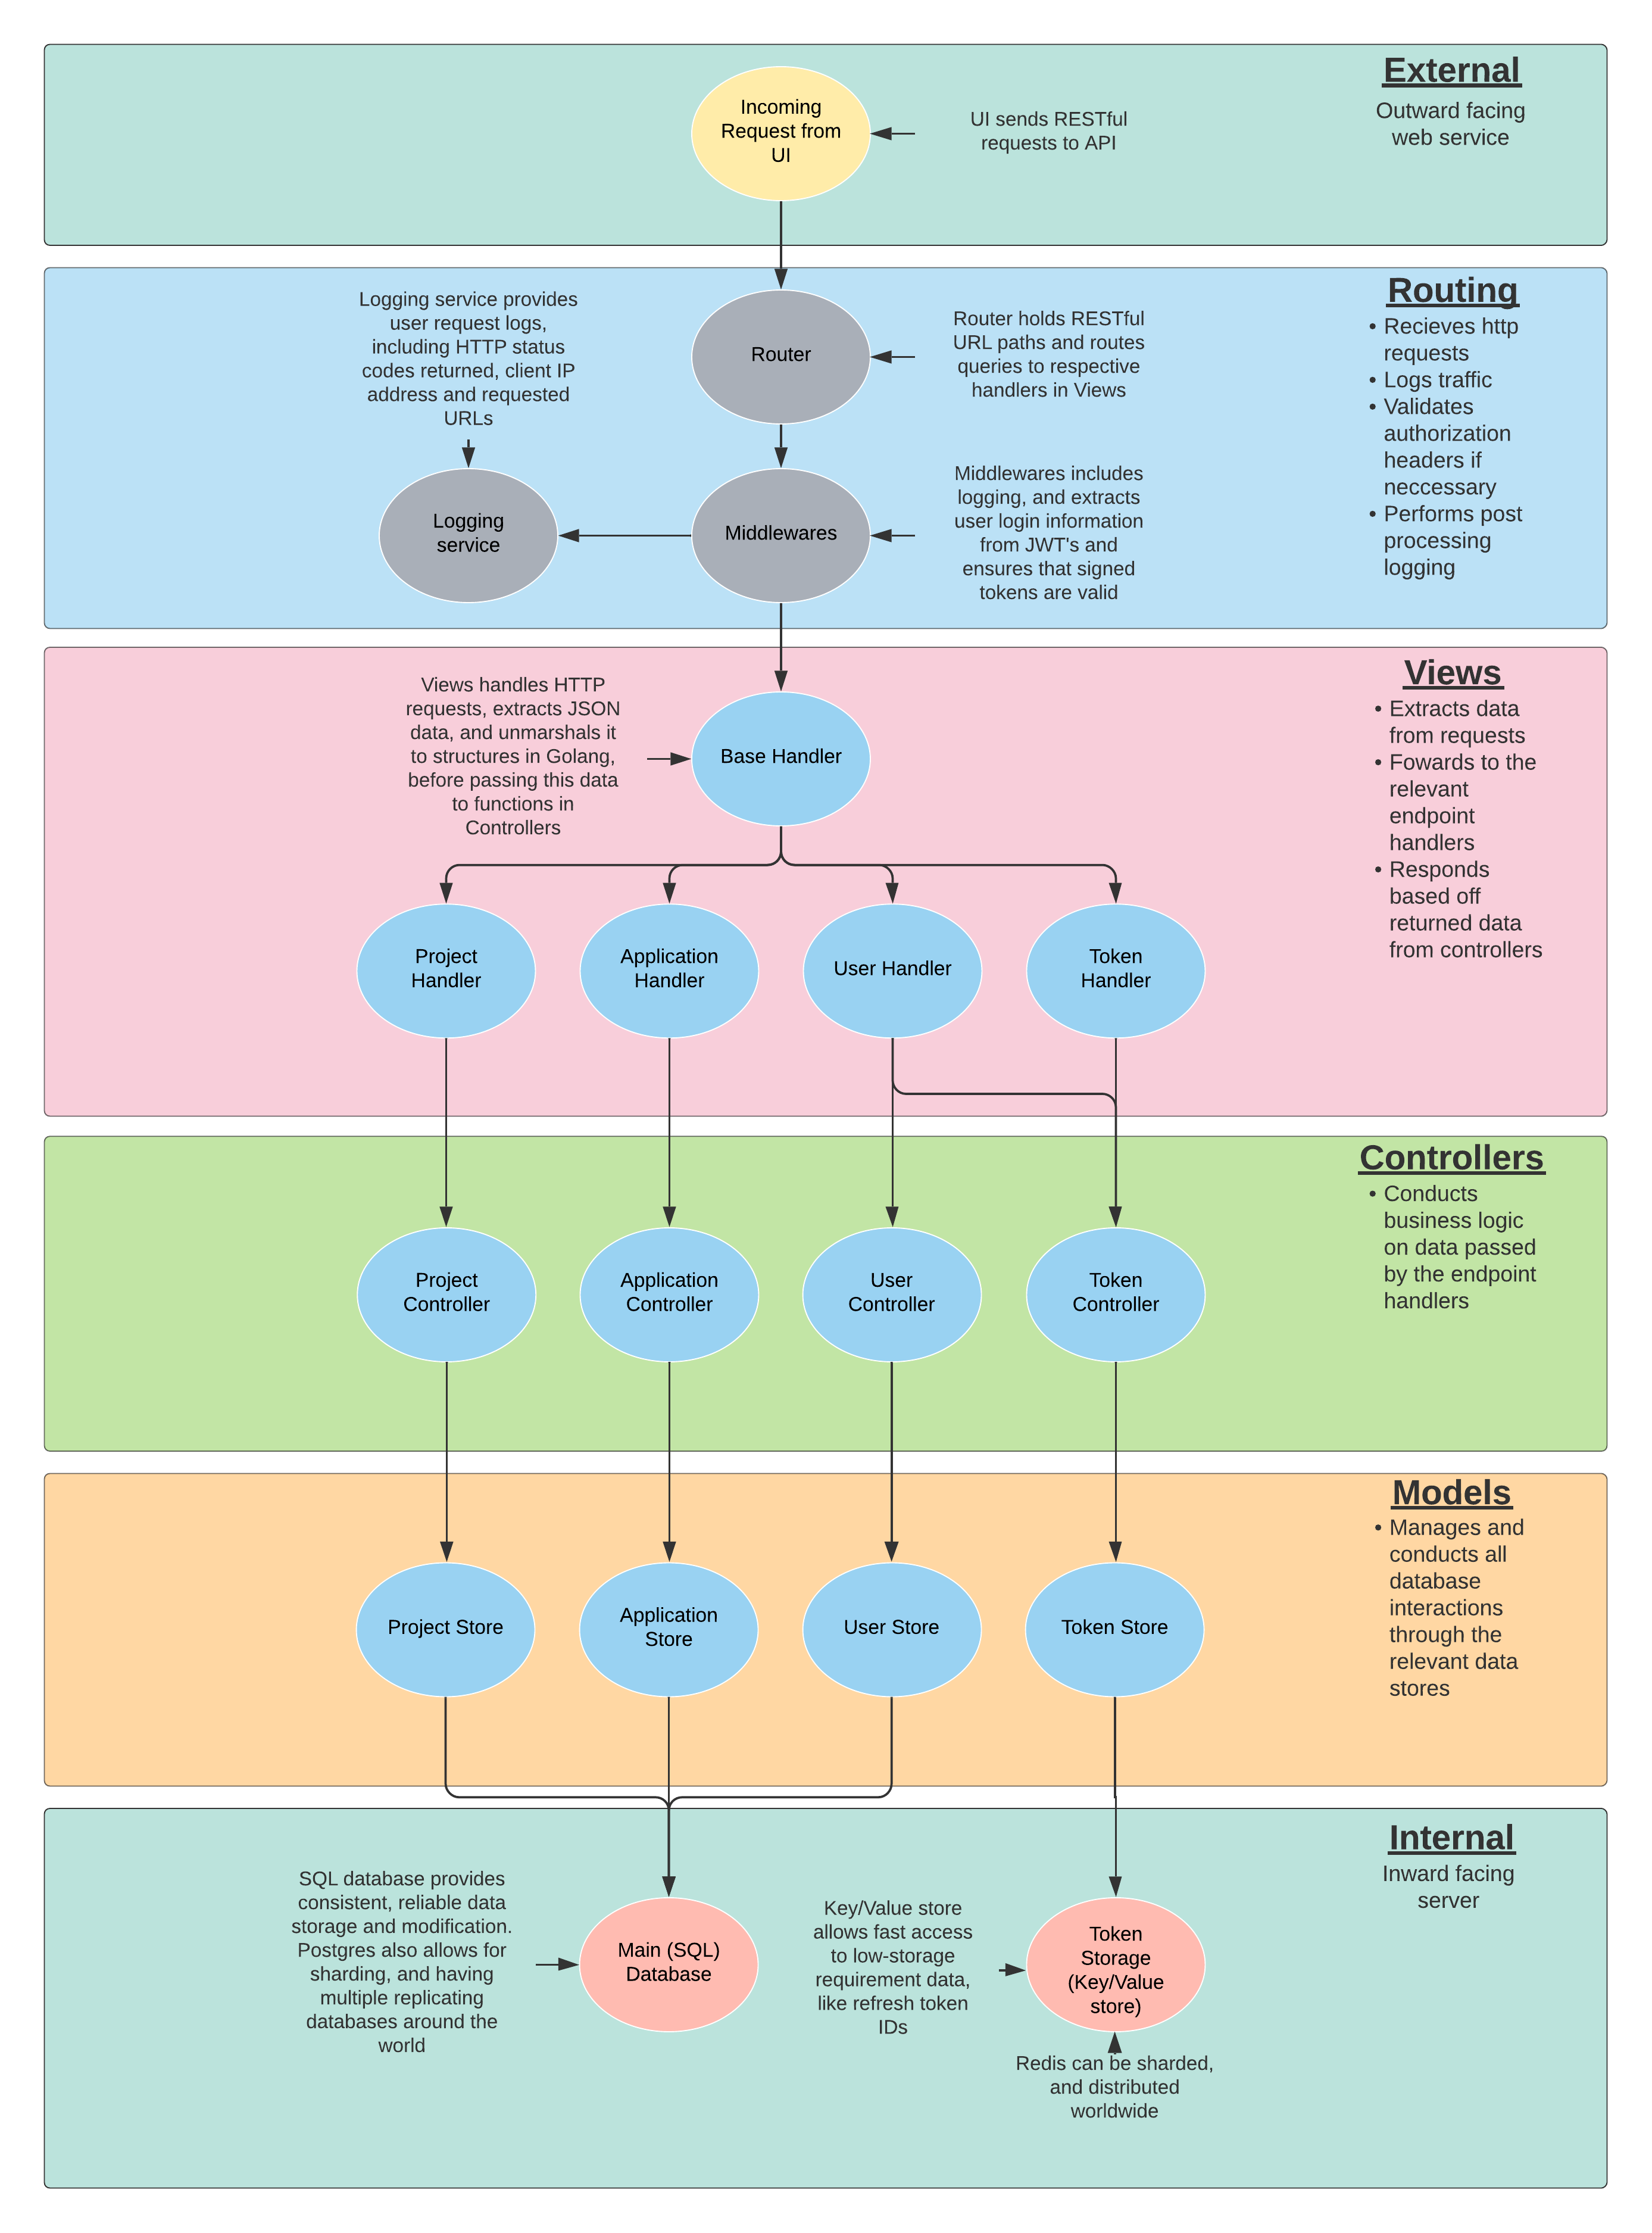
\includegraphics[width=\textwidth,keepaspectratio]{backend-overview.png}
    \caption{Backend Overview}
    \label{fig:backend-overview}
\end{figure}

\section{Router}
A router is a process that takes in a request and depending on the data in the
request, decides which handler is used to handle the request. With this, we can
have separate handlers for each API interaction, and allows for RESTful request
parameters in the requested URL (eg. /users/{id}, where id is ther user's ID
number).

\section{Middleware}
Middleware is a process that is used between routing and handling of the route.
It can also be used (as in our case) to call on the handler, and run some code
before and after a request is handled. In so doing, we can run authentication
middleware before handling the request, and perform logging once the request is
handled.

\subsection{Authentication Middleware}
This middleware inspects the HTTP request "Authorization" header, and checks the
token. We use JWTs \footnote[1]{JSON Web Tokens} to encode and store a digital
fingerprint in a user's access token. In this JWT, we store a user's ID. If the
token has expired, or has been tampered with (ie. encrypted header and claims of
JWT do not match the signed string), then a user is not authenticated, and user
ID is not passed into the request context.

\subsection{Logging}
As this middleware can run code before and \textbf{after} a request is handled,
we can assess what the response to the request detailed, including HTTP status
code, whether the request was considered a "success", or an "error", the
client's IP address, and the request HTTP method, and path. This logging will be
output to STDOUT

\section{Views}
The Views process contains all of the handlers, split up into sub-processes
depending on the context of the resource to be accessed. These request handlers
simply unmarshal request data and send this data to controllers with
instructions on what to do with it.

\section{Controllers}
Controllers take data and instructions from handlers in Views, and modifies and
structures data to be ready to write/read from the database. It then sends this
data to the relevant data store to write/read to the database.

\section{Stores}
Stores provides an abstract interface to the database, allowing a controller to
make a very simplified, concise request to modify data by sending a pointer to
data. This pointer's value gets modified by the Store after data is
fetched/modified on database.

\section{Database}
The database holds information, and is either a SQL relational database, or a
key/value store, depending on the resource. Authorization token IDs are stored
in the key/value store, and everything else is stores on the SQL relational
database.

\chapter{Project Approach}
We believe scrum is the best solution for our team. The scrum project management
structure allows for the prioritisation of more important tasks. Self-delegation
is important to us, to allow us to work on tasks we are most effective on. Scrum
identifies problems in the project earlier than waterfall, which helps in
prioritising a functional product. The strict time schedule for scrum is also
very useful as we have other time commitments to other modules and out of
college activities. We believe we can use our close communication ties to
minimise the issues of task progress identification. A strong issue with
waterfall is the late realisation of bugs and issues in the timeline of the
project; possibly rewriting important code late into the stage. For these
reasons we think scrum is the better option for our team.

\chapter{Deliverable 2 Minutes}

\section{Meeting \#1}

\begin{flushright}
    Date: 18/10/2021

    Time: 6pm

    Location: Online via Discord
\end{flushright}

\Large{Attendance:}
\normalsize

\begin{itemize}
    \item Aidan
    \item Thomas
    \item Max
    \item Shang
    \item Reece
\end{itemize}

Coordinator: Thomas

\vspace{1cm}

\Large{Second Deliverable duties}
\normalsize

\begin{itemize}
    \item Market Research - Max \& Aidan
    \item Finalize required implementation details - Thomas \& Reece
    \item State-Transition Diagrams - Thomas \& Reece
    \item Data-Flow Diagram - Thomas \& Reece
    \item Sequence Diagram - Shang
\end{itemize}

\vspace{0.5cm}

\Large{Additional Duties to Undertake}
\normalsize
\begin{itemize}
    \item Implementation Documentation - Thomas \& Reece
\end{itemize}

\newpage
\section{Meeting \#2}

\begin{flushright}
    Date: 21/10/2021

    Time: 6pm

    Location: Online via Discord
\end{flushright}

\Large{Attendance:}
\normalsize

\begin{itemize}
    \item Aidan
    \item Thomas
    \item Max
    \item Shang
    \item Reece
\end{itemize}

Coordinator: Thomas

\vspace{1cm}

\Large{Duties to complete}
\normalsize
\begin{itemize}
    \item Market Research - Max \& Aidan
    \item Data-Flow Diagram - Thomas
    \item State-Transition Diagrams - Thomas \& Reece
\end{itemize}

\vspace{0.5cm}

\Large{Additional Duties to undertake}
\normalsize
\begin{itemize}
    \item Backend Overview - Thomas \& Reece
    \item Wireframes - Max \& Shang
    \item ER Diagrams - Reece
\end{itemize}

\chapter{GANTT Chart}
\begin{figure}[h]
    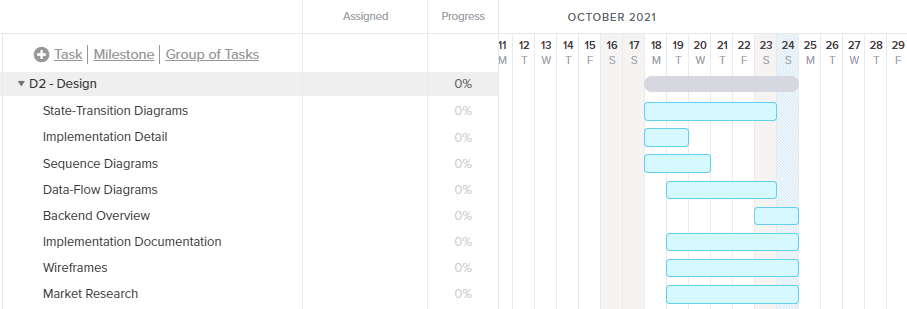
\includegraphics[width=\textwidth,keepaspectratio]{gantt.png}
\end{figure}

\end{document}